% Chapter 4, version 5 (23 September 2026). Revised from annotated 04V4.tex.
% The accompanying appendix 04_AppendixV3.tex retains labels app:clean-metrics,
% app:clean-resnet and app:clean-trufor. Tables may be relocated to it later.
% Requires graphicx, booktabs, tabularx, array, amsmath and the master's
% citation setup. Existing figure: Images/CH04_Restoration_V1.png.
% Face/text author review is in progress. Joint E/RRA thresholds, DCEC counts
% and a separate restoration-artifact classifier result are NOT established.

\chapter{Clean Performance and Spatial Evidence Audit}
\label{ch:clean}

\section{Why clean evidence matters}
\label{sec:clean-purpose}

The question in this thesis is what happens to a useful spatial map when an adversary changes the image but leaves a correct forgery decision intact. Hence it is imperative to establish which clean decisions are correct and whether their maps point to the altered regions. ``Clean'' here means \emph{before the additional adversarial perturbation}; the document may already contain an edited face or text field.

This chapter addresses following objectives. 
\begin{itemize}
    \item O1 by measuring document decisions and spatial agreement for both pipelines.
    \item O2 by checking a compression shortcut and testing which edited regions influence model's decision.
\end{itemize}

It reports the clean DC (decision correct) population and the continuous map measures from which DCEC (decision correct, evidence correct) will be drawn. A final DCEC count is also provided using a joint evidence thresholds and visual review. This distinction keeps failures that occur \emph{before} an attack visible.

The details of the spatial measures and review procedure are in Appendix~\ref{app:clean-metrics}. ResNet and TruFor decisions, alternatives and residual risks are documented in Appendices~\ref{app:clean-resnet} and~\ref{app:clean-trufor}. Chapter~3 describes how the evaluated pipelines were built, including ResNet's ImageNet initialisation, classifier-head training and subsequent full fine-tuning.

\section{Images, splits and evaluation conditions}
\label{sec:clean-scope}

FantasyID supplies photographed documents and annotations of the altered regions \citep{korshunov2025fantasyid}. It has a total of 3,284 images split into training(1,899) and test(1,385) dataset. The open 1,899-image training release was divided by document stem into 1,440 images from 160 card-stems for this project's training and 459 images from 51 different stems for project development. The public release dataset audit established the units, dependencies and family semantics required for valid interpretation of the experiments.”Figure~\ref{fig:FantasyIDdatasetEval} describes the process with discovered features about the dataset while Figure~\ref{fig:FantasyIDdatasetAudit} shows auditory information derived. This \emph{internal} development split must not be confused with the separately released, restricted FantasyID validation set, which was not used due to its EULA restrictions.
% The official test contains 1,385 images: 786 Digital-3, 150 FaceDancer, 149 TextDiffuserFT-BFEI and 300 bona fide. Related captures of the same card are linked by stem when making the project split and during uncertainty estimation.

\begin{figure}[H]
% \centering
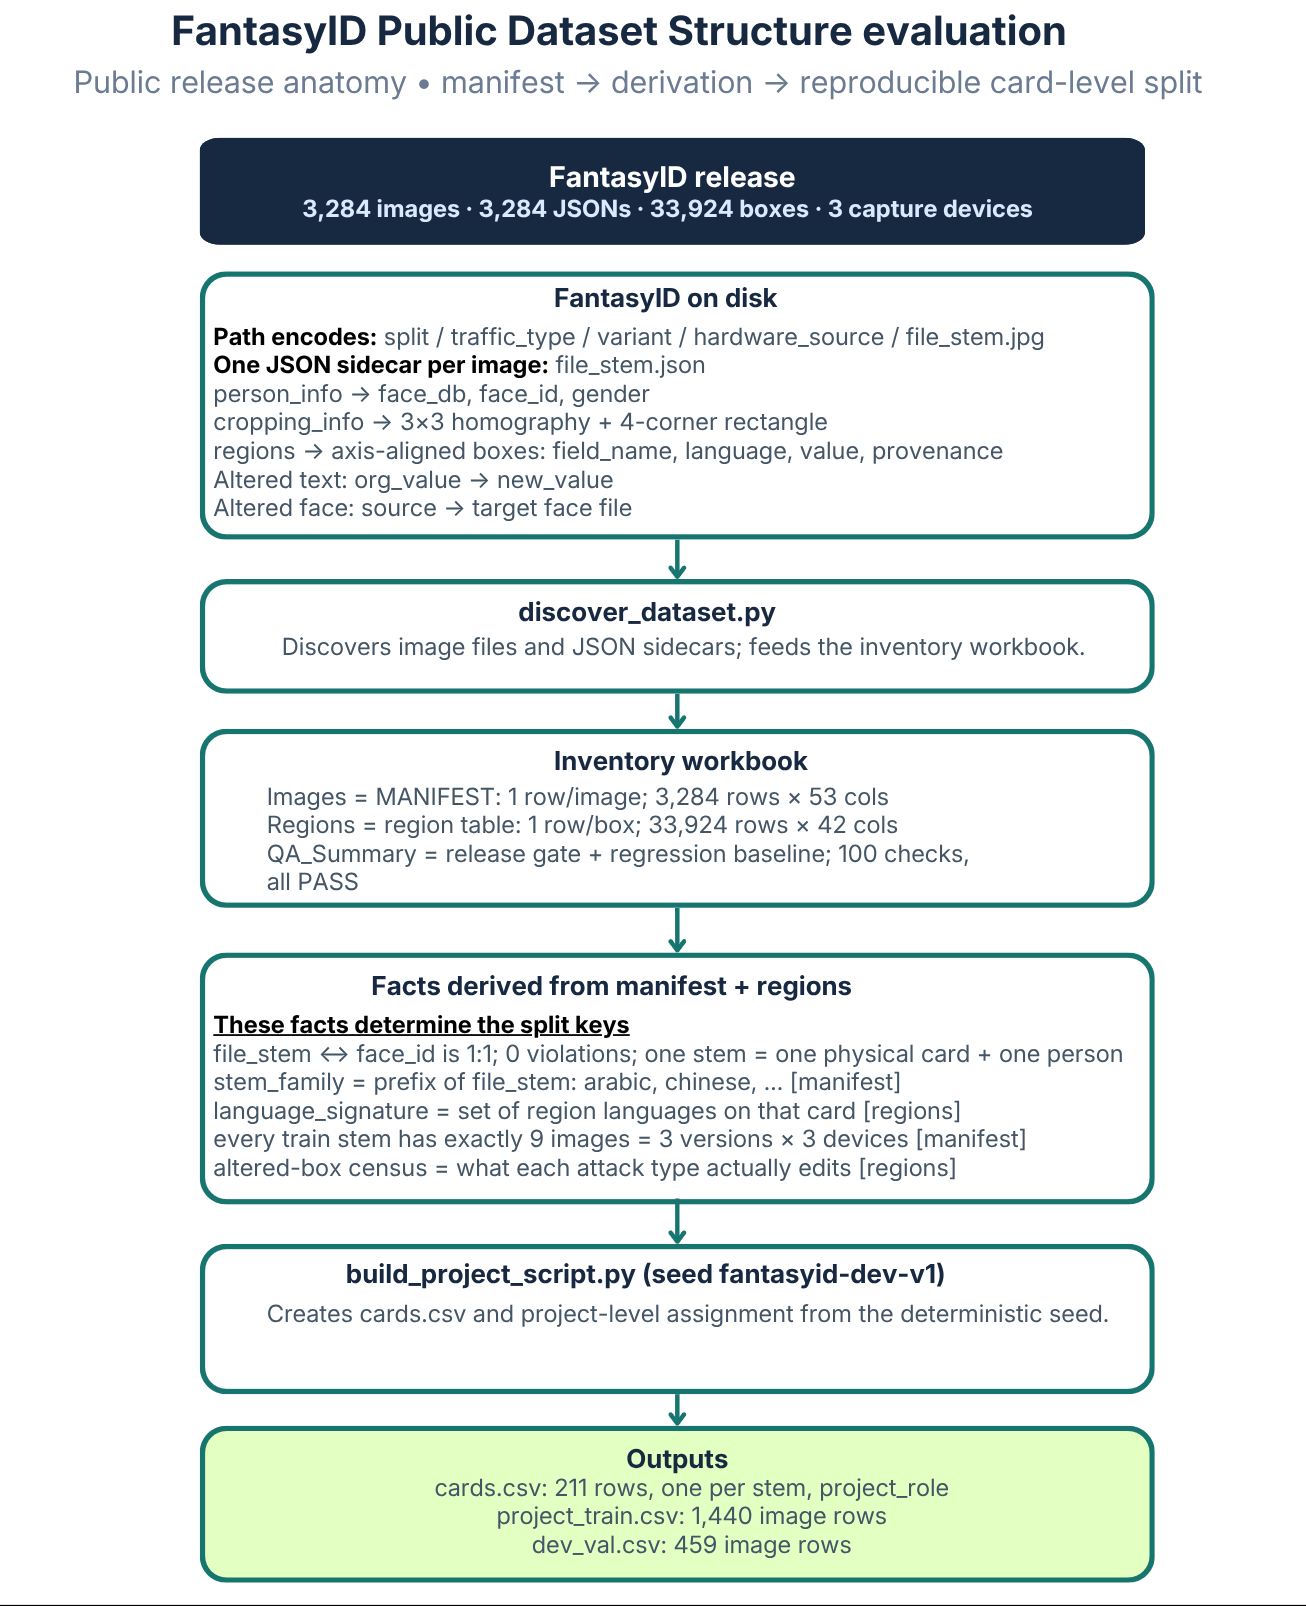
\includegraphics[width=0.95\textwidth,height=0.73\textheight,keepaspectratio]{Images/CH04_01.png}
\caption{Evaluation process of Fantasy ID dataset along with discovered information.}
\label{fig:FantasyIDdatasetEval}
\end{figure}

\begin{landscape}
\thispagestyle{empty}

\begin{figure}[H]
\centering
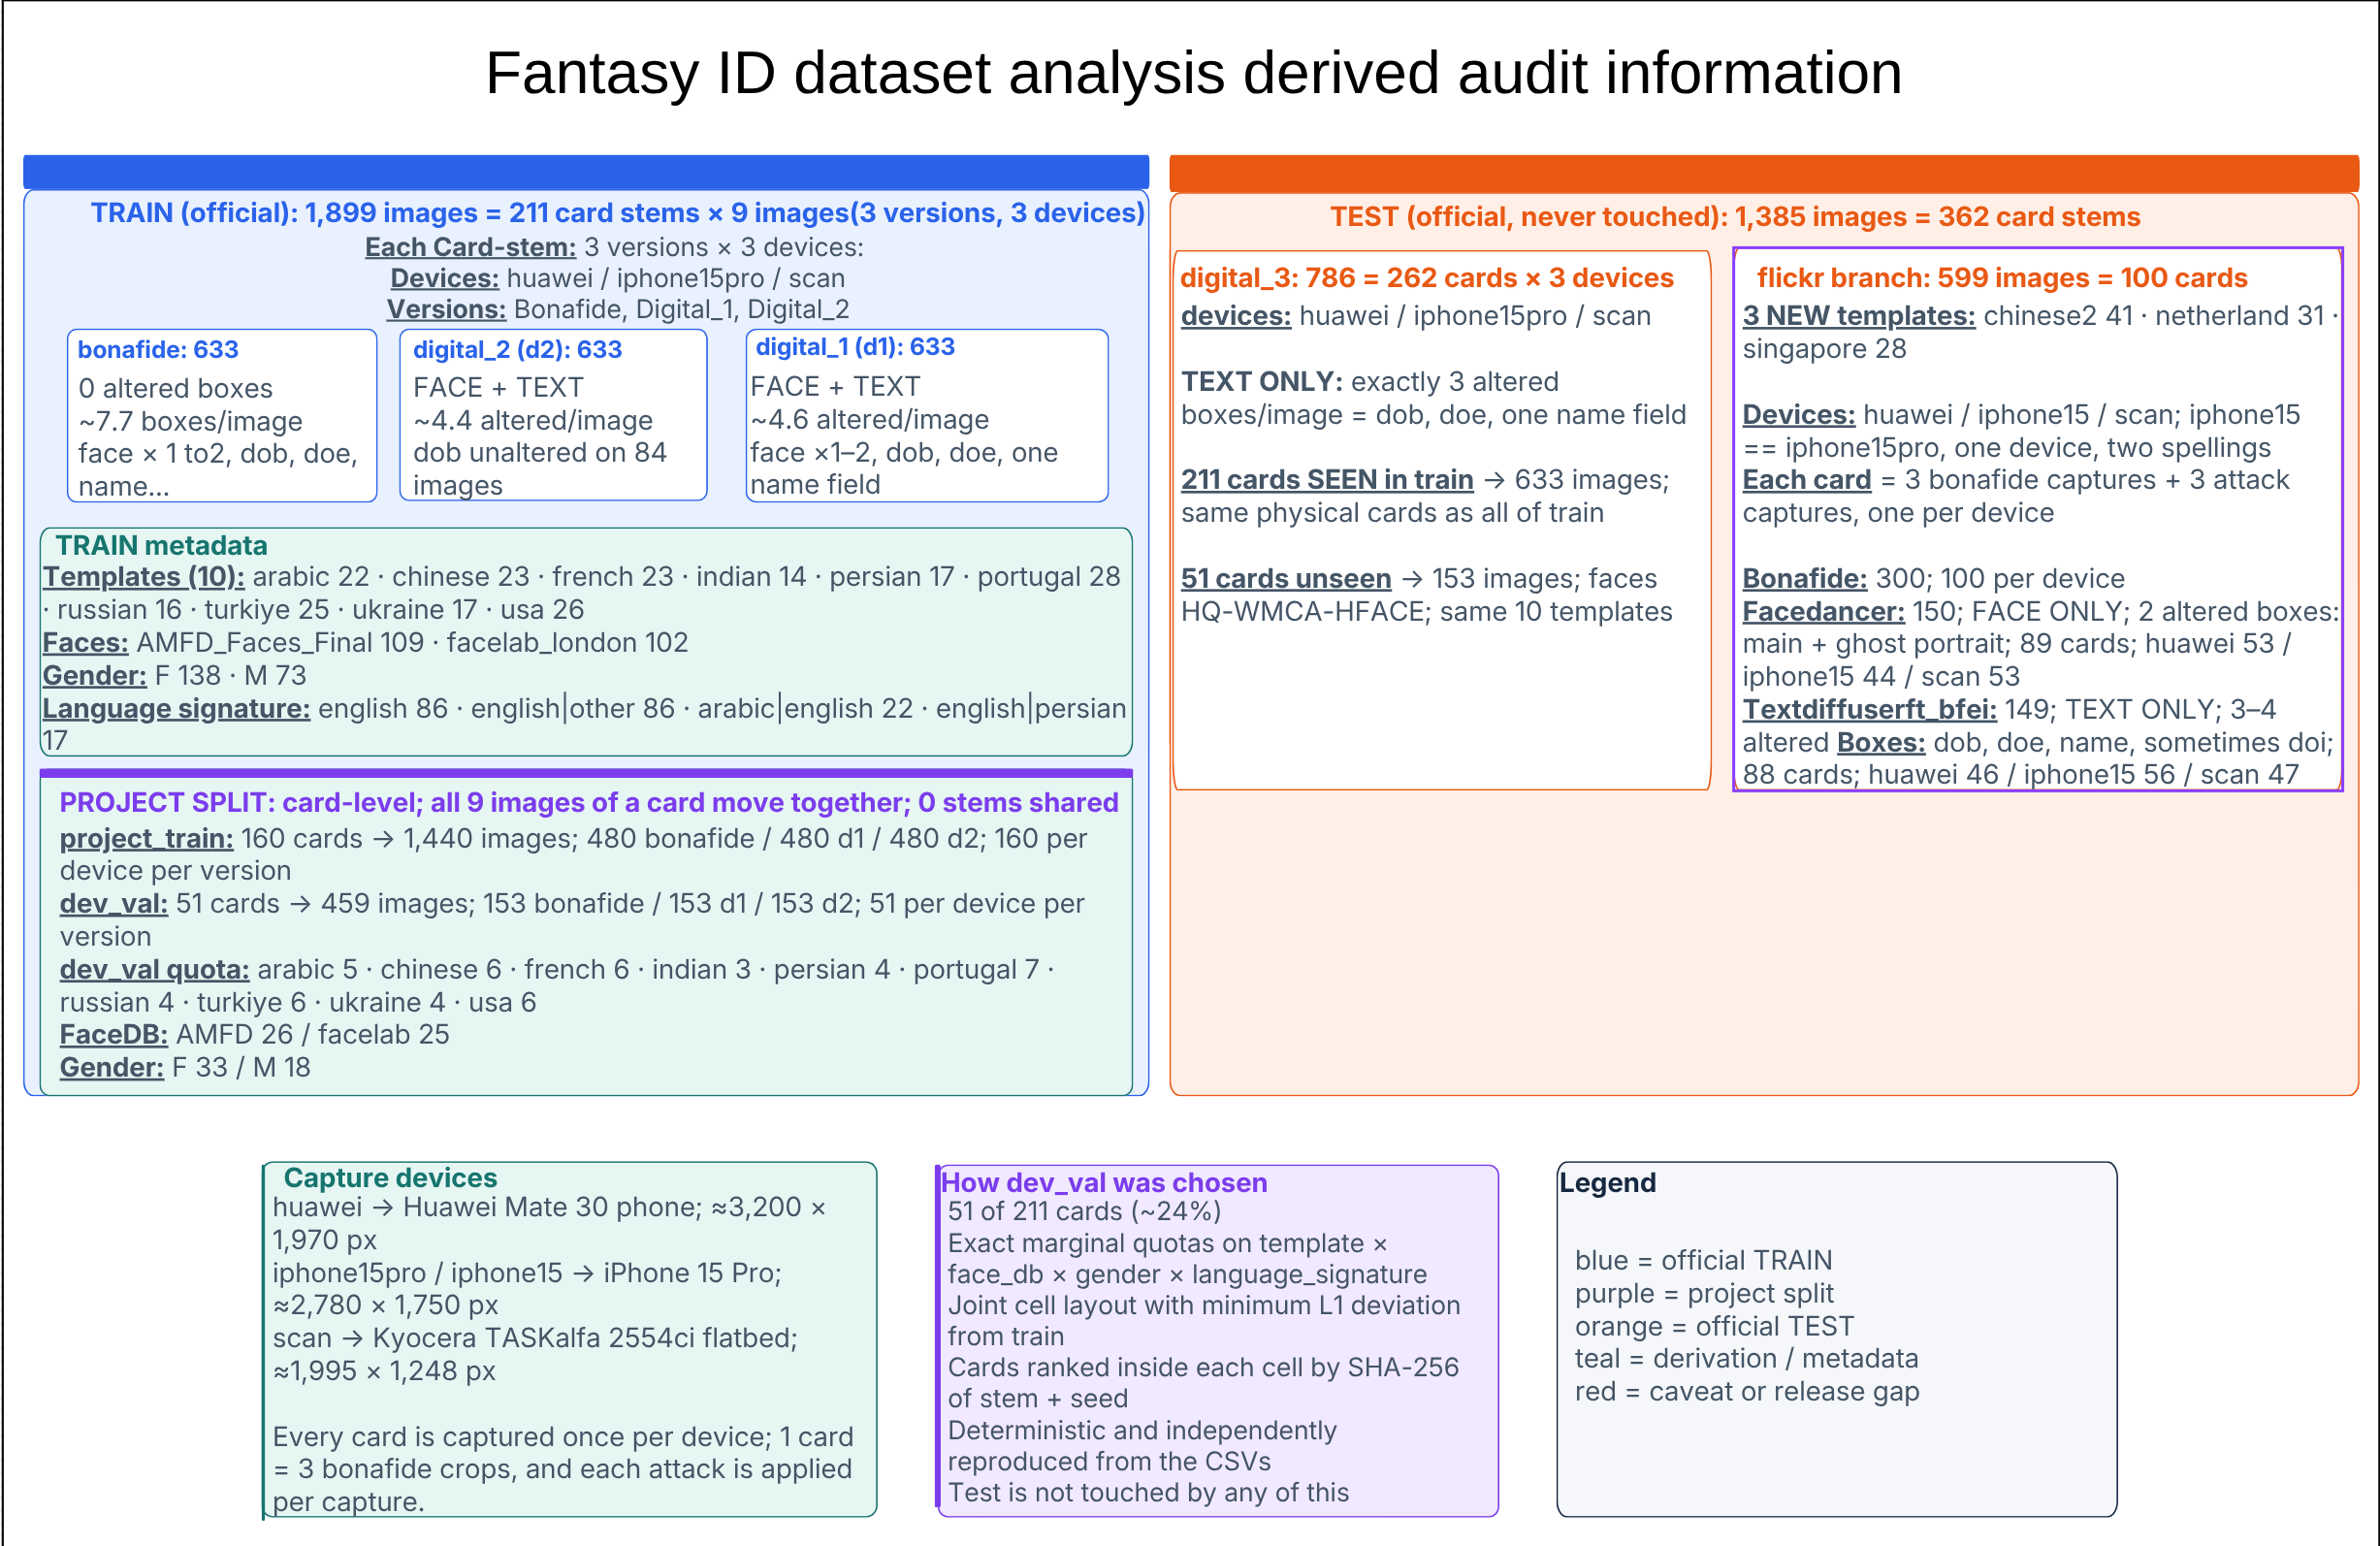
\includegraphics[
    width=1.0\linewidth,
    height=0.8\textheight,
    % keepaspectratio
]{Images/CH04_02_Dataset_Audit.png}
\caption{Fantasy ID dataset audit information.}
\label{fig:FantasyIDdatasetAudit}
\end{figure}

% Landscape page number
\begin{tikzpicture}[remember picture,overlay]
\node[rotate=90] at ([xshift=1.25cm]current page.west) {\thepage};
\end{tikzpicture}

\end{landscape}

ResNet-18 was trained on Digital-1 and Digital-2 categories and receives a resized document within a padded canvas. Grad-CAM is calculated from the forged-minus-bona-fide logit at the last residual block. TruFor keeps its pretrained weights, reads the document at its original resolution and produces a map of manipulation likelihood. Its \emph{decision} threshold was selected using the project-development images; its weights were not adapted in the final condition. ``Zero-shot'' therefore describes the weights, not an absence of calibration. 
%sa-review
% An earlier fine-tuning trial followed a different evaluation protocol and is recorded in Appendix~\ref{app:clean-trufor}, not merged with these results.

The development results are partly apparent performance: they informed ResNet checkpoint selection and TruFor threshold calibration. The official test prompted some later diagnostics, which are identified below as post-hoc checks. Training exposure, image resolution, map meaning and calibration all differ between pipelines. The main question remains how each pipeline's spatial output holds up against \emph{its own} clean baseline.

\section{Checking the compression shortcut}
\label{sec:clean-shortcut}

An initial audit found an alternative explanation for very good development detection. JPEG-history features alone separated forged from bona-fide development images with AUROC 1.000. The audit fitted a simple \emph{logistic-regression classifier} on compression features from project training, then tested it on the stem-disjoint development set. It showed that preparation history could reveal the class without examining the edited face or field. This is the kind of shortcut discussed in Chapter~2 \citep{geirhos2020shortcut}.

Policy C was adopted to reduce this class-correlated cue. Table~\ref{tab:clean-policy-c} gives the actual image sequence; the two JPEG encodings are separate, with a decode between them. The final quality is deterministic for a document stem and capture source, so its forged and bona-fide versions receive the same assignment. Chapter~3 and Appendix~\ref{app:clean-resnet} give the implementation and the reasons for choosing this policy.

\begin{table}[htbp]
\centering\small
\caption{Policy C at a glance. The same final quality is assigned to images from the same card and capture source. This is an outline of the implemented sequence, not a new image enhancement method.}
\label{tab:clean-policy-c}
\begin{tabularx}{\textwidth}{@{}lp{0.30\textwidth}X@{}}
\toprule
Step & Input and operation & Output \\
\midrule
1 & Decode the source JPEG to RGB. & Source pixels in memory. \\
2 & Encode those pixels as JPEG at quality 75, 4:2:0. & Common intermediate JPEG. \\
3 & Decode the intermediate JPEG to RGB. & Intermediate pixels in memory. \\
4 & Encode at a deterministic, matched quality from 50 to 90, 4:2:0. & Generates the Policy-C image used in evaluation. \\
\bottomrule
\end{tabularx}
\end{table}

Using the same kind of logistic-regression probe after this control,following was observed. 
\begin{itemize}
    \item Final JPEG-table features alone gave development AUROC 0.500.
    \item Broader JPEG-history features gave 0.524.
    \item All measured compression features together gave 0.586, with a stem-resampled 95\% interval [0.572, 0.606].
\end{itemize}
These are \emph{different feature sets}, not three scores for one unchanged input. The aim was to harmonise a preparation cue correlated with the class, not to remove every encoding trace a real edit might leave.

Both evaluated pipelines use Policy-C images. Recompression could weaken a useful forensic trace, while residual histories could still influence a decision. The results describe this controlled condition, not performance on the source files or in a bank. The regional intervention below, tests whether ResNet also responds to edited content under the control. It cannot restore traces lost through recompression or exclude every shortcut. These limits are retained in the Appendix~\ref{app:clean-resnet} risk register.

\section{Document decisions across forgery families}
\label{sec:clean-detection}

DeepID competition style overall reporting provides a useful first view: it includes false alarms on genuine cards as well as missed forgeries. Table~\ref{tab:clean-pooled} uses class-weighted F1, as in the competition's detection reporting, alongside accuracy, balanced accuracy and the underlying correct counts \citep{korshunov2025deepid}. These are \emph{this study's} Policy-C results at its chosen decision thresholds. They are not challenge leaderboard scores: the inputs and TruFor threshold differ from the challenge protocol, and the private competition set was not evaluated here. DeepID also scores binary localisation masks; the spatial measures later in this chapter answer a different question.

\begin{table}[htbp]
\centering
\small
\setlength{\tabcolsep}{4.5pt}
\caption{Pooled clean detection under this study's protocol. ``Forged DC(Decision-Correct)'' and ``BF(Bona-fide) correct'' give the numerators and denominators behind the summary. Accuracy, balanced accuracy (BA), class-weighted F1 and AUROC are calculated separately for each split.}
\label{tab:clean-pooled}

\begin{tabular}{@{}ll|cc|rrrr@{}}
\toprule
Split & Pipeline & Forged DC & BF correct & Accuracy & BA & Weighted F1 & AUROC \\
\midrule

Dev & ResNet-18 & 306/306 & 148/153 & .989 & .984 & .989 & 1.000 \\
Dev & TruFor & 288/306 & 73/153 & .786 & .709 & .769 & .843 \\
\midrule

Test & ResNet-18 & 182/1,085 & 209/300 & .282 & .432 & .274 & .234 \\
Test & TruFor & 1,042/1,085 & 131/300 & .847 & .699 & .831 & .944 \\

\bottomrule
\end{tabular}
\end{table}

An overall figure as noted in Table~\ref{tab:clean-pooled} and used in competitions cannot show \emph{which} kind of forgery a model detects or whether its spatial map points to the edit. Table~\ref{tab:clean-detection} therefore retains the family results. AUROC is the chance that a randomly selected forgery receives a higher forgery score than a randomly selected genuine document, across decision thresholds. Each family AUROC uses that family's forgeries and the bona-fide pool from the \emph{same split}. DC and balanced accuracy refer instead to the selected operating threshold. Balanced accuracy is $(\text{forged recall}+\text{bona-fide specificity})/2$; the same genuine pool is reused for each family in a split. 
%sa-review
% It should not be confused with the forged-only DC population used for spatial evidence.

\begin{table}[htbp]
\centering
\small
\setlength{\tabcolsep}{4.5pt}
\caption{Clean detection by forgery family. Forged $n$ is the original family size. DC is the number correctly called forged; BA includes genuine images from the same split. All results use the final fixed decision thresholds.}
\label{tab:clean-detection}

\begin{tabular}{@{}llr|rrr|rrr@{}}
\toprule
 & & &
\multicolumn{3}{|c}{ResNet-18} &
\multicolumn{3}{|c}{TruFor} \\
\midrule

Split & Family & Forged $n$
& AUROC & DC/$n$ & BA
& AUROC & DC/$n$ & BA \\
\midrule

Dev & Digital-1 & 153 & 1.000 & 153/153 & .984 & .986 & 153/153 & .739 \\
Dev & Digital-2 & 153 & 1.000 & 153/153 & .984 & .699 & 135/153 & .680 \\
\midrule

Test & Digital-3 & 786 & .059 & 6/786 & .352 & .999 & 786/786 & .718 \\
Test & FaceDancer & 150 & .958 & 144/150 & .828 & .601 & 107/150 & .575 \\
Test & TextDiffuserFT & 149 & .429 & 32/149 & .456 & .999 & 149/149 & .718 \\

\bottomrule
\end{tabular}
\end{table}

ResNet's 6/786 Digital-3 decisions and 32/149 TextDiffuser decisions reveal a much narrower test population for later evidence analysis than the pooled number suggests. 
TruFor detects every Digital-3 and TextDiffuser image here, but at its fixed threshold it also flags 169 of the 300 genuine test cards. 

High AUROC on those families describes score ranking however it does not undo the false-positive rate. The large Digital-3 family can also dominate a pooled score while a smaller family behaves differently.

ResNet uses a forged-score threshold of 0.5. TruFor uses one threshold, 0.532956, selected on development images for every family and capture source. 
%sa-review
% These classification thresholds are distinct from the two, still-unfrozen requirements for acceptable spatial evidence. Table~\ref{tab:clean-trufor-threshold} shows the trade-off against TruFor's upstream 0.5 operating point. The selected threshold improved apparent development accuracy and genuine specificity but missed five more forgeries. It was fitted to equal-weight image accuracy on these development images, not to a bank's cost of accusing a genuine customer.
These classification thresholds are distinct from the requirements for acceptable spatial evidence. Table~\ref{tab:clean-trufor-threshold} shows the trade-off against TruFor's upstream 0.5 operating point. The selected threshold improved apparent development accuracy and genuine specificity but missed five more forgeries. It was fitted to equal-weight image accuracy on these development images, not to a bank's cost of accusing a genuine customer.

\begin{table}[htbp]
\centering
\small
\setlength{\tabcolsep}{5pt}
\caption{TruFor development decisions at two fixed thresholds. The selected threshold was fitted on these same 459 images; the table is a calibration diagnostic, not independent validation. AUROC is unchanged because the score order does not change.}
\label{tab:clean-trufor-threshold}

\begin{tabular}{@{}l|cc|rrr@{}}
\toprule
Forged-score threshold & Forged DC & BF correct & Accuracy & BA & Weighted F1 \\
\midrule

Upstream .500 & 293/306 & 51/153 & .749 & .645 & .714 \\
Selected .532956 & 288/306 & 73/153 & .786 & .709 & .769 \\

\bottomrule
\end{tabular}
\end{table}

The one TruFor threshold also behaves unevenly across development capture sources (Table~\ref{tab:clean-trufor-device}). For Huawei captures, only five of 51 genuine cards are accepted; the corresponding number for iPhone15Pro is 41 of 51. The groups are small and related through card identities. No device-specific threshold was fitted after seeing this spread.

\begin{table}[htbp]
\centering\small
\caption{TruFor development results by capture source at the single selected threshold. Source-specific BA uses only that source's forged and bona-fide images; each group contains 102 forgeries and 51 genuine cards.}
\label{tab:clean-trufor-device}

\begin{tabular}{@{}l|cc|cc@{}}
\toprule
Capture source & Forged DC & BF correct & BF specificity & BA \\
\midrule
Huawei & 99/102 & 5/51 & 9.8\% & .534 \\
iPhone15Pro & 96/102 & 41/51 & 80.4\% & .873 \\
Scan & 93/102 & 27/51 & 52.9\% & .721 \\
\bottomrule
\end{tabular}
\end{table}

\section{Does ResNet respond to the edited regions?}
\label{sec:clean-regions}

For ResNet, the development score were near perfect but test scores did not match up to that. Further, the development forgeries contain altered face and text regions, whereas the unseen families in test dataset change the mix of manipulations. The uneven decisions above raised a practical question of whether ResNet-18 learnt cues from both kinds of region edits(face, text), or mainly from one? 
A larger face edit might be easier for a whole-document classifier to learn than a small text change, but that is a hypothesis, not an explanation supplied by the detection scores. Hence the regional test was designed to examine that possibility.

% Optional explanatory image to add when its annotation and edit-family
% descriptions have been checked against the actual FantasyID family records.
% Suggested file: Images/CH04_Family_Edit_Contrast_V1.pdf.
%sa-review
\IfFileExists{Images/CH04_Family_Edit_Contrast_V1.pdf}{%
\begin{figure}[htbp]
\centering
\includegraphics[width=0.94\textwidth]{Images/CH04_Family_Edit_Contrast_V1.pdf}
\caption{Illustrative face and text annotations in the development families and examples from unseen test families. The panels illustrate edit scale; they are not a measurement of why a classifier succeeds or fails.}
\label{fig:clean-family-edits}
\end{figure}
}{}

For each suitable development image, the annotated face or text was replaced with the corresponding region from the same card's bona-fide capture. Geometry and JPEG processing were matched. Figure~\ref{fig:clean-restoration} reports the average of ResNet's forged-class scores \emph{over the same paired cards} before and after replacement. This shows score movement even when both scores lead to the same class decision; it is neither a localisation score nor a calibrated probability of fraud.

\begin{figure}[htbp]
\centering
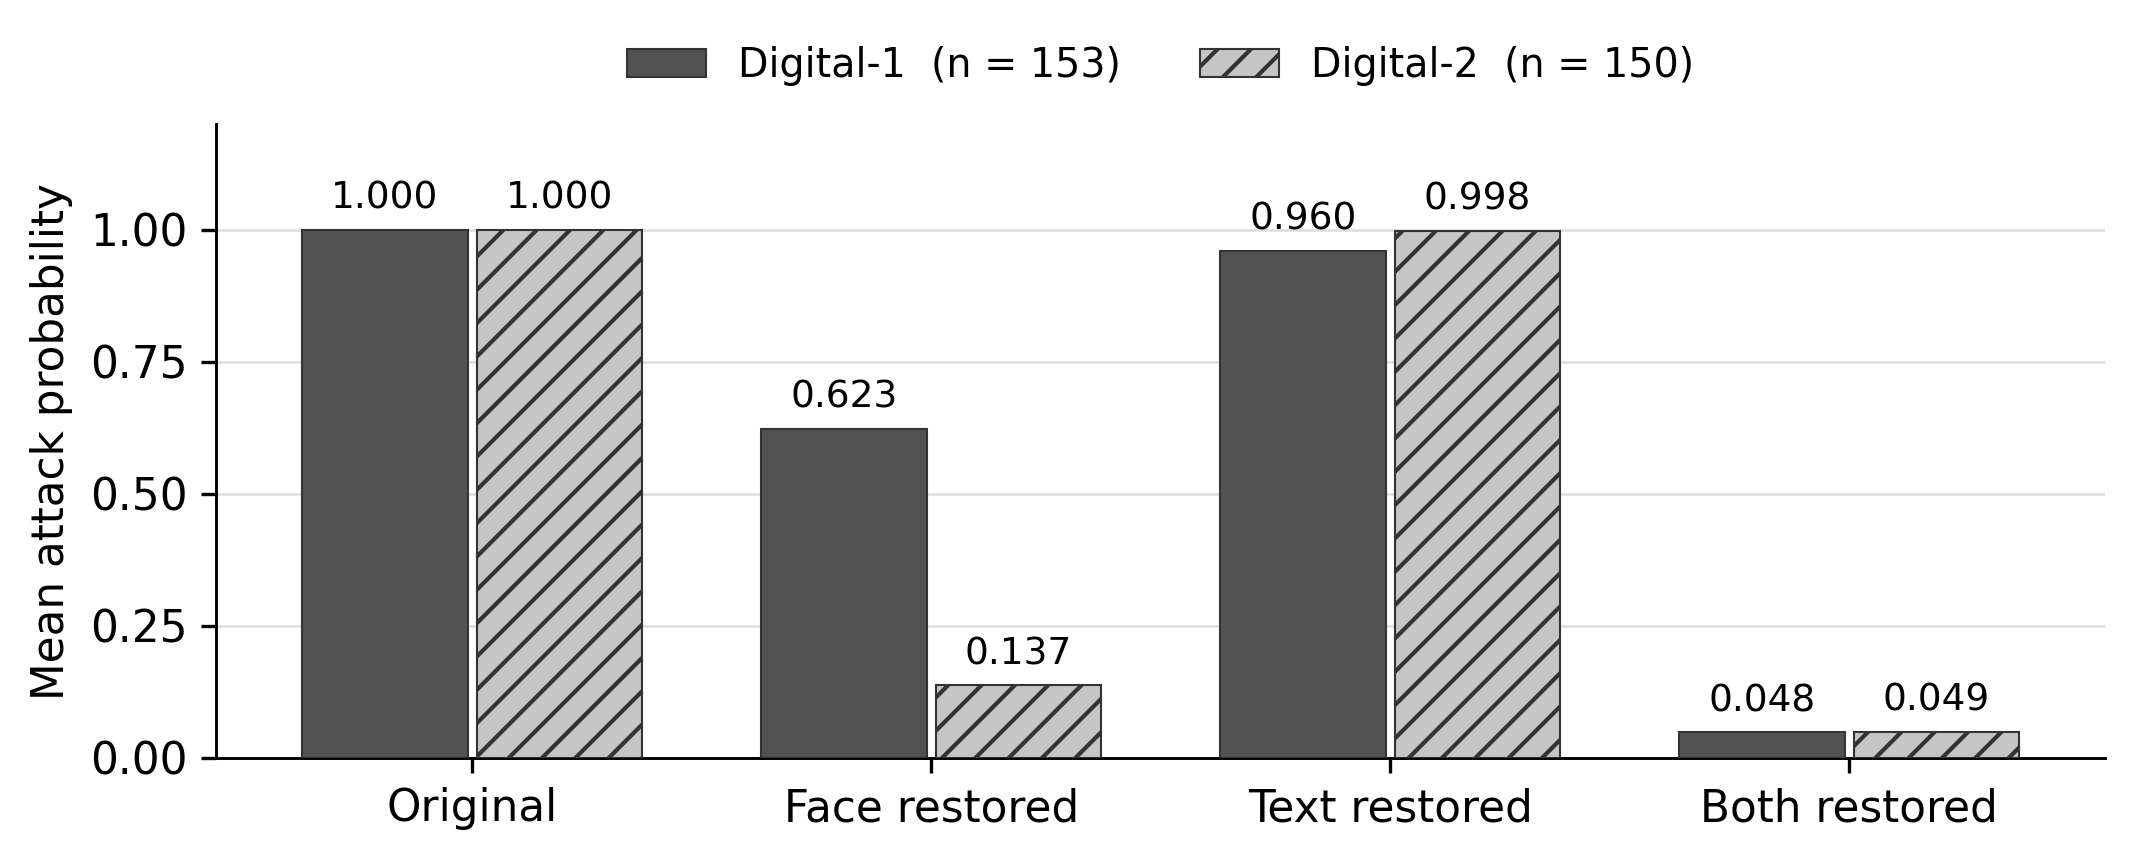
\includegraphics[width=0.96\textwidth]{Images/CH04_Restoration_V1.png}
\caption{Mean ResNet forged-class scores after same-card regional restoration on development images. Digital-1 uses 153 pairs; Digital-2 uses 150 because three pairs have incompatible geometry. Bars describe paired image-score averages, not the effect of a single isolated forensic feature.}
\label{fig:clean-restoration}
\end{figure}

On Digital-2 from development dataset, the mean score falls from almost 1.000 to 0.137 when the face is restored, but remains 0.998 when only text is restored. Restoring both regions brings it near the genuine-card score of 0.049. This supports stronger dependence on face-region content under the tested intervention. 

It does not prove that text never matters or reveal the exact texture used. Replacement can also change local boundaries. Although the procedure matches JPEG processing and geometry, a separate classifier test of post-restoration artifacts was also performed. Its results evidence that post-restoration artifacts were not enough to separate out post-restoration artifacts.
%sa-review
Altered boundaries still remain a residual risk in Appendix~\ref{app:clean-resnet}. A restoration-augmented training trial improved some internal cue balance but left official-test AUROC at 0.089 for Digital-3 and 0.463 for TextDiffuser. It was a diagnostic, not the primary model regardless.

Digital-3 from test dataset required another check. In 153 pairs, an \emph{official-test Digital-3 forgery} was matched to the bona-fide parent card in this project's development data. The forgery's score rose relative to its own parent in 82.4\% of pairs. Yet the average increase was only 0.0094 and its stem-resampled interval included zero; the same-source AUROC was 0.628 [0.592, 0.669]. The official-test AUROC of 0.059 instead compares all 786 Digital-3 forgeries with a different pool of 300 official-test bona-fide cards. These checks suggest that a weak response to the edit and a change in the comparison population could both matter. They do not identify a single proven cause, and the paired check was pursued after the official-test result was seen purely as diagnostics.

\section{Agreement between maps and altered regions}
\label{sec:clean-spatial}

Chapter~2 introduced altered-area fraction $A$ (Area) and $E$ as the Relevance Mass Accuracy (RMA). $E$ is the fraction of map mass inside the annotated region; $A$ is the fraction of valid document area it occupies. The ratio $\mu_w=E/A$ expresses how concentrated the map is relative to that area's size. If a map spreads its mass evenly, $E$ is close to $A$. 

The Pointing Game (PG) asks only whether the \emph{single strongest} map pixel falls inside an annotated region. Relevance rank accuracy (RRA) checks how many of the strongest pixels, selected in the same number as the altered pixels, lie inside it. Appendix~\ref{app:clean-metrics} specifies the per-image calculations and invalid-map rules.

Table~\ref{tab:clean-spatial} keeps three denominators visible: the original forged family, its clean DC subset and the maps evaluated. All displayed map summaries are now restricted to DC. In particular, the archived ResNet FaceDancer audit covered all 150 maps; this table filters its individual-image records to the 144 correctly detected images, so its means differ slightly from the earlier whole-family description. ResNet excludes its artificial padding when calculating map agreement. TruFor uses its native manipulation map. 
%sa-review??????????????????????????????
A common-coordinate RRA audit still needs to be completed before setting the final evidence gate.

\begin{table}[htbp]
\centering\small\setlength{\tabcolsep}{5pt}
\caption{Clean spatial agreement, conditional on a correct forgery decision. ``All'' is the original family size, ``DC'' the correctly detected count and ``maps'' the number summarised. $A$ is altered document area in percent; $E$ and PG are fractions. The displayed $\mu_w$ is the mean of per-image $E_i/A_i$, not the ratio of the displayed means. ResNet's FaceDancer row is calculated from its per-image records after filtering to DC.}
\label{tab:clean-spatial}
\begin{tabular}{@{}llr|rr|r|rrr@{}}
\toprule
Map & Family & All $n$ & DC $n$ & Maps $n$ & $A$ (\%) & $E$ & $\mu_w$ & PG \\
\midrule
Grad-CAM & Digital-1 (dev) & 153 & 153 & 153 & 15.9 & .707 & 4.77 & 1.000 \\
Grad-CAM & Digital-2 (dev) & 153 & 153 & 153 & 9.3 & .546 & 6.16 & .523 \\
\midrule
Grad-CAM & Digital-3 (test) & 786 & 6 & 6 & 2.6 & .0007 & .03 & .000 \\
Grad-CAM & FaceDancer (test) & 150 & 144 & 144 & 6.6 & .494 & 7.82 & .722 \\
Grad-CAM & TextDiffuserFT (test) & 149 & 32 & 32 & 4.3 & .010 & .24 & .000 \\
\midrule
\addlinespace

TruFor & Digital-1 (dev) & 153 & 153 & 153 & 15.7 & .555 & 3.90 & 1.000 \\
TruFor & Digital-2 (dev) & 153 & 135 & 135 & 9.3 & .192 & 2.09 & .504 \\
\midrule
TruFor & Digital-3 (test) & 786 & 786 & 786 & 2.9 & .642 & 23.26 & .991 \\
TruFor & FaceDancer (test) & 150 & 107 & 107 & 6.9 & .112 & 1.70 & .402 \\
TruFor & TextDiffuserFT (test) & 149 & 149 & 149 & 4.2 & .703 & 17.13 & 1.000 \\
\bottomrule
\end{tabular}
\end{table}

The ``means'' help describe a family, but can hide how varied its individual maps are. Table~\ref{tab:clean-spatial-median} gives the median and middle half of the image-level $E$ values behind the preceding table. These are descriptive distributions for DC images, not DCEC pass rates.

\begin{table}[htbp]
\centering\small
\caption{Median relevance mass $E$ and interquartile range (IQR) among the DC images in Table~\ref{tab:clean-spatial}. Values are computed from per-image map records; RRA thresholds are not inferred from this table.}
\label{tab:clean-spatial-median}
\begin{tabular}{@{}ll|c|c@{}}
\toprule
Map & Family & Median $E$ & $E$ IQR \\
\midrule
Grad-CAM & Digital-1 (dev) & .708 & [.639, .784] \\
Grad-CAM & Digital-2 (dev) & .520 & [.467, .624] \\
Grad-CAM & Digital-3 (test) & .00032 & [.00005, .00150] \\
Grad-CAM & FaceDancer (test) & .531 & [.367, .581] \\
Grad-CAM & TextDiffuserFT (test) & .00266 & [.00031, .01199] \\
\addlinespace
TruFor & Digital-1 (dev) & .550 & [.406, .693] \\
TruFor & Digital-2 (dev) & .157 & [.112, .232] \\
TruFor & Digital-3 (test) & .697 & [.453, .859] \\
TruFor & FaceDancer (test) & .102 & [.084, .124] \\
TruFor & TextDiffuserFT (test) & .778 & [.579, .860] \\
\bottomrule
\end{tabular}
\end{table}

\newpage
%sa-review add image!!!!
An ID can have both a changed face and changed text. A high $E$ over the \emph{combined} annotation could still come entirely from the face. A PG success only establishes that one peak falls somewhere inside that combined area. Table~\ref{tab:clean-components} therefore separates the face and text contributions on the two development families. For Digital-2, ResNet places an average 0.540 of its total map mass in the face region but only 0.006 in text, even though its union $E$ is 0.546. Its strongest point is in the combined annotation in only 80 of 153 cases. The component results expose what the union summary misses.

\begin{table}[htbp]
\centering\small
\caption{Mean share of total map mass in the annotated face and text regions on correctly detected development forgeries. The union is the existing $E$ measure; component results are shown because a union-level score need not cover both edits. Face and text annotations can overlap, so their shares need not add exactly to the union.}
\label{tab:clean-components}
\begin{tabular}{@{}llr|rrr@{}}
\toprule
Map & Dev family & DC maps $n$ & Face $E$ & Text $E$ & Union $E$ \\
\midrule
Grad-CAM & Digital-1 & 153 & .658 & .049 & .707 \\
Grad-CAM & Digital-2 & 153 & .540 & .006 & .546 \\
\midrule
TruFor & Digital-1 & 153 & .359 & .197 & .555 \\
TruFor & Digital-2 & 135 & .161 & .031 & .192 \\
\bottomrule
\end{tabular}
\end{table}

ResNet's FaceDancer maps (test) show meaningful concentration on the edited area when restricted to the 144 DC images; its six correctly detected Digital-3 maps (test) and 32 TextDiffuser maps (test) show very little. Six Digital-3 examples cannot represent that 786-image family. 

TruFor gives stronger clean spatial agreement on Digital-3 and TextDiffuser but weaker agreement on FaceDancer. 

These differences describe the \emph{implemented pipelines}, with different outputs and resolutions. The attack question compares each one to its own starting maps, so no claim that one architecture is inherently better is needed.

For the \emph{mean $E$} values in Table~\ref{tab:clean-spatial}, ResNet's Digital-1 and Digital-2 development rows have document-stem-resampled 95\% intervals [0.677, 0.736] and [0.513, 0.578], respectively. They describe sampling variation across these document stems for this fitted model. They do not include a new training seed or uncertainty in the annotation rectangles. Neither means nor medians can tell us how many individual maps pass both eventual $E$ and RRA requirements.

\section{Visual review and the unfinished evidence gate}
\label{sec:clean-review}

The supplied rectangles approximate a manipulation, and an enlarged Grad-CAM map is coarse. A visual check is therefore needed alongside numeric agreement. The author is reviewing development maps against the altered document and its same-card bona-fide reference. Face and text are rated separately, with an ambiguous category where a yes/no judgement would overstate what can be seen. The ongoing coding task uses the displayed images and maps rather than per-image $E$, RRA, proposed DCEC membership or attack outcomes. Appendix~\ref{app:clean-metrics} gives the coding sheet, sampling procedure and intended threshold-selection rule.

This is an \emph{author-conducted contextual review}. The author has seen some aggregate results before rating the images, so it cannot be presented as an independent or prospectively blind assessment. Consistent display rules and a repeat rating of selected images can help expose inconsistent judgements; they cannot turn those judgements into ground truth or show how a document examiner would use a map. Ratings, agreement statistics and the final joint $E$/RRA thresholds remain incomplete at this version.

The order of work must also be disclosed. Attacks were first run on the broader DC population, before the clean-evidence rule was finalised. The remaining control is to choose the evidence rule from clean development measurements and the declared visual ratings, without optimising it against attack success. Official-test results, attack outcomes and a convenient eligible sample size must not select the thresholds. Prior analyst exposure remains a limitation. Appendix~\ref{app:clean-metrics} records the sensitivity checks needed before a DCEC claim, including coordinate conventions, uncertain rectangle boundaries and component coverage.

\section{What the clean population supports}
\label{sec:clean-populations}

Across the five manipulated families, ResNet has 488 observed DC images and TruFor has 1,330. These totals combine the development and official-test family counts in Table~\ref{tab:clean-detection}; they are \emph{not} evidence-eligible sample sizes. For each pipeline, the eventual DCEC gate will retain DC images whose clean $E$ and RRA both meet its accepted thresholds. The same accepted thresholds must then be used on that pipeline's attacked maps. Until calibration and coordinate checks finish, no DCEC coverage or shared-DCEC intersection can be reported.

The full denominator trail is original forged family $\rightarrow$ clean DC $\rightarrow$ clean DCEC. Low coverage at any stage will be reported, not hidden by reporting success only among eligible examples. Within the fixed DCEC set, DCEW means the attack makes spatial evidence fail while the forgery decision stays correct. A classification flip remains in the original DCEC denominator but is reported separately. The existing attacks on DC images can be analysed again under the later clean-only eligibility rule without rerunning them. Images eligible for both pipelines may provide matched visual examples and another view of \emph{within-pipeline} degradation; their intersection is not a controlled architecture comparison.

\section{Conclusion}
\label{sec:clean-conclusion}

The clean audit shows why a correct document decision is only a first step. ResNet's very strong development detection does not carry evenly to unseen forgery families, and its Digital-2 map is concentrated mainly on the face. TruFor has different strengths across families and many false alarms on genuine official-test cards at its selected threshold. The compression and regional checks narrow some alternative explanations while leaving documented risks. Objective O1 now has a clear detection and continuous spatial baseline; O2's author review and joint evidence calibration are still under way. Chapter~5 will assess adversarial evidence degradation against each pipeline's fixed clean DCEC population once that population is established.
